\chapter{Nonrelativistic Quantum Electrodynamics}

\section{Effective Field Theories}
The most generally powerful approach to nonrelativistic bond state theories is the use of the techniques of effective field theory.  In this chapter we develop the theory of such an approach.


\subsection{Brief background}
First, a brief background of the development of effective field theories.

The first workable relativistic theory of quantum mechanics came from Dirac.  By realising that a relativistic equation for fermions necessitated a four component spinor, he was able to write down what is now known as Dirac's equation.  This led to the prediction of the electron's antiparticle the positron.

The relativistic theory necessitated the introduction of an infinite degrees of freedom.  Thus, wave functions had to be promoted to fields, and the first quantum field theory arose.  It was highly successful at predicting leading order quantities, but when attempting to use perturbation theory within this context, a number of infinities arose.

To resolve this matter, QED and renormalization were developed in the late 1940s.  The key was in changing the parametrization from of the theory from ``bare'' values, to measured values at some particular energy scale.  So to completely define the theory one needed to write down not only the Lagrangian but also the renormalization point.  The coupling constants of the theory would depend upon this.  With this approach QED was enormously successful, producing very accurate predictions to such quantities as the anomalous magnetic moment.

There was much frustrating work to formulate a theory of the other interactions along the same lines.  During this work (such as that by Gell-man and Low) with these types of theories it became clear that there was structure to how the coupling constants behaved as the renormalization point changed.

While working through the Ising model, Wilson, who had a background working with QFTs, realised there were applications of these renormalisation ideas to critical phenomena.    Later, working with fixed-source meson theory, had an insight that led to effective field theory.  Working with a hierarchy of momentum ``slices'' and a process of eliminating energy scales, he found that although an infinite number of interactions was generated, the effects at each iteration were bounded -- only a finite number of terms were necessary for any particular level of precision.  A successful theory with arbitrarily many constants still worked, as long as there was a clear hierarchy of terms.

An effective field theory was not renormalizable in the way QED was, but as Wilson found the proliferation of terms could be contained such that only a finite number mattered for a particular calculation.  The constraint is that an effective field theory has application only well below some energy scale.  But, the very feature that it is formulated at a particular scale makes it in many ways the natural theory to use at that scale.


\subsection{A Worked example of Renormalization}
Let us review how the process of renormalization works when a theory {\it is} renormalizable.
%TODO Define what a cut-off actually is

%TODO Make sure to mention locality of terms!

The QED Lagrangian defined at some cut-off is:
\beq
	\mathcal{L}_0 = 
		\bar{\Psi} \left( i \partial \cdot \gamma - e_0 A \cdot \gamma - m_0 \right) \Psi - \frac{1}{4} F^{\mu\nu}) F^{\mu\nu} 
\eeq 
and additionally the cut-off regulator $\Lambda_0$.  

In calculating a process without a cut-off, all intermediate states must be summed over.  When kinematics do not strictly dictate the intermediate momenta of some particles, this means integrating over an infinite range.  This is exactly the case with an internal loop (as it described in the language of Feynman diagrams), and is what caused the infinities that plauged initial attempts to formulate relativistic quantum mechanics. 

By introducing a cut-off, the integrals only take place over a bounded domain of momenta, and are thus finite.  The cost is that physical quantities should not depend upon this arbitrary cut-off $\Lambda_0$.  Still, the parameters can be fixed by comparing with experiment.  This theory will then produce results correct up to some terms of $\mathcal{O}(1/\Lambda_0^2)$.

There are two parameters: the mass $m_0$ and the bare charge $e_0$.  These parameters are determined from experiment.  Two processes can be calculated (such as electron-electron scattering and the electron scattering off some external field), compared to the experimental measurements, and thus the parameters fixed.

Handed this theory with a high cut-off $\Lambda_0$, it is possible to reformulate it in terms of a new, lower cut-off $\Lambda$.  The new theory will hold valid for processes where the external momenta are much less than $\Lambda$.	

By introducing this lower cut-off, high energy virtual processes are eliminated from the theory.  Rather than being explicitly included, their effects will implicitly be included by corrections to the parameters of the theory.

These corrections can be calculated from the original theory.  Before, loop-integrals over momenta ran from $0$ to the old cut-off $\Lambda_0$.  In the new theory, they will run from $0$ to $\Lambda$.  Clearly the difference between the two calculations will be an integral from $\Lambda$ to $\Lambda_0$.  Importantly, because $\Lambda$ is taken to be greater than the energy of any process considered, so will the loop momentum in that sector of the integral.

%TODO insert diagram of vertex correction
First consider the calculation of the electron vertex.  Call the original value $T$, which will have contributions from several diagrams.  On such contribution is from the one loop diagram, where a photon is exchanged between the fermion line before and after the interaction.  Call this contribution $T^{(a)}$.  

In the original $\mathcal{L}_0$ theory the contribution would be
\beq
	T{(a)}(k>0) = -e_0^3 \int_{0}^{\Lambda_0} \frac{d^4 k}{(2\pi)^4} \frac{1}{k^2} \left\{
		\bar{u}(p') \gamma^\mu \frac{1}{(p'-k) \cdot \gamma -m_0} A_{\text{ext}}(p'-p) \cdot \gamma \frac{1}{(p-k) \cdot \gamma -m_0} \gamma_\mu
		u(p) \right\}
\eeq  


When the momenta are cut-off at the lower point $\Lambda$, the part of the old integral missing from the new calculation will be
\beq
	T{(a)}(k>\Lambda) = -e_0^3 \int_{\Lambda}^{\Lambda_0} \frac{d^4 k}{(2\pi)^4} \frac{1}{k^2} \left\{
		\bar{u}(p') \gamma^\mu \frac{1}{(p'-k) \cdot \gamma -m_0} A_{\text{ext}}(p'-p) \cdot \gamma \frac{1}{(p-k) \cdot \gamma -m_0} \gamma_\mu
		u(p) \right\}
\eeq  
Remember that $\Lambda$ is chosen to be a great deal greater than $p$, $p'$ or $m_0$, and this then holds for $k$ over the entire range of the integral.  Then, if corrections of the type $p/\Lambda$ are discarded, the integral can be greatly simplified.  The approximation used is:

\beq
	\frac{1}{(p'-k) \cdot \gamma -m_0} \approx -\frac{1}{k \cdot \gamma}
\eeq
Of course for any four vector $a$, it holds that $(a \cdot \gamma)^2 = a^2$, so
\beq
	-\frac{1}{k \cdot \gamma} = - \frac{ k\cdot \gamma}{k^2}
\eeq
Then
\beqa
T^{(a)}(k>\Lambda) 
	&\approx&  -e_0^3 \int_{\Lambda}^{\Lambda_0} \frac{d^4 k}{(2\pi)^4} \frac{1}{k^2}  \left\{
			\bar{u}(p') \gamma^\mu \frac{ k\cdot \gamma}{k^2} A_{\text{ext}}(p'-p) \cdot \gamma \frac{ k\cdot \gamma}{k^2} \gamma_\mu
		u(p) \right\}	\\
	&\approx&	-e_0^3 \bar{u}(p')  A_{\text{ext}}(p'-p) \cdot \gamma u(p) 
				\int_{\Lambda}^{\Lambda_0} \frac{d^4 k}{(2\pi)^4} \frac{1}{k^4}  
\eeqa
	
There are other one electron scattering diagrams.  When the above analysis is applied to them all, the total difference is found to be of the form:

\beq
T^(k>\Lambda) = -ie_0 c_0( \Lambda / \Lambda_0 ) \bar{u}(p')  A_{\text{ext}}(p'-p) \cdot \gamma u(p) 
\eeq	
This is the piece of the electron vertex structure that we are missing if we calculate using the original Lagrangian with the lower cut-off.  The correct results will be obtained if we incorporate into the Lagrangian a new term:
\beq
	\delta \mathcal{L} = -e_0 c_0( \Lambda / \Lambda_0 ) \bar{u}(p')  A_{\text{ext}}(p'-p) \cdot \gamma u(p) 
\eeq

What about the nature of this constant $c_0$?  Consider the above calculation of $T^{(a)}(k>\Lambda)$.  It had, like the total correction, had a structure of some constant terms times $ \bar{u}(p')  A_{\text{ext}}(p'-p) \cdot \gamma u(p) $.  The structure of the constant term came from the integral over a function of only $k$.  Since there were no scales involved in this integration, other than the limits of integration, the result must be some function of $\Lambda$ and $\Lambda_0$.  And because the integral is dimensionless, it must actually be a function of their ratio $\Lambda / \Lambda_0$.  The same logic goes through when the other terms are computed.  The final result is that
\beq
	c_0 =  - \frac{\alpha_0}{6\pi} \log(\Lambda / \Lambda_0 )
\eeq


That the result of these integrals involves only the limits is contingent upon the approximation made earlier, that the scales $p$, $p'$ and $m_0$ are all small compared to $\Lambda$.  If corrections of that order are important, then there will be additional terms with structures including these momenta and mass.  This can be accomplished by, instead of completely neglecting these terms, doing Taylor expansion in terms of $p/k$, $m_0/k$ and so forth.  We'll return to this later. %TODO check k vs. lambda for expansion  

Going back to the correction $\delta \mathcal{L}$, note that it has almost the same form as a term in the original $\mathcal{L}_0$, the difference being an explicit dependence on the cut-offs $\Lambda$, $\Lambda_0$.  (Although of course, $e_0$ itself depended on comparing measurements to calculations in the $\mathcal{L}_0$ theory, so it really {\it was} dependent on $\Lambda_0$.)  Rather than interpret it as new interaction, then, it can be seen as change in the strength of $e_0$.  

\beq
 - \bar{\Psi} e_0 A \cdot \gamma  \Psi \to - \bar{\Psi} e_0  [1 + c_0(\Lambda/\Lambda_0) ] A \cdot \gamma  \Psi
\eeq 

As long as all other scales are considered to small to $\Lambda$ to enter the calculations, it isn't possible for truly new terms to enter, only corrections to the already existing terms.  That means that all that can happen is an adjustment of the existing coupling constants $e_0$ and $m_0$.

There are indeed corrections to $m_0$, coming from the electron self-energy.  An additional correction term is required of the form
\beq
	\delta \mathcal{L} = - m_0  \tilde{c}_0(\Lambda/\Lambda_0) \bar{\Psi} \Psi
\eeq

The Lagrangian valid with the new cut-off $\Lambda$ can be written in terms of the old as:
\beq
	\mathcal{L}_\Lambda = 
		\bar{\Psi} \left( i \partial \cdot \gamma - e_\Lambda A \cdot \gamma - m_\Lambda \right) \Psi - \frac{1}{4} F^{\mu\nu}F_{\mu\nu} 
\eeq 
where the constants are
\beqa
	e_\Lambda &=& e_0 (1 + c_0)				\\
	m_\Lambda &=& m_0 (1 + \tilde{c}_0)
\eeqa


Above only two processes were considered, which produced corrections to known interactions.  In principle corrections will also arise from other processes, such as electron-electron scattering.

But, consider the form of such cross-sections.  They must have a spinor structure something like $\bar{u}u \bar{u} u$ or $\bar{u}\gamma^\mu u \bar{u} \gamma_\mu u$, with an accompanying factor.  Certainly it involves four fermion fields.  The key point is that the scattering amplitude with four external lines must be dimensionless.  Since $u$ has mass dimension $1/2$, $d_0$ must have dimension $-2$.  

So to write a dimensionless factor $d_0$ analogous to $c_0$ above, there must be an additional factor of mass dimension $-2$.  The relevent scale is $\Lambda$, so this factor must be $1/\Lambda^2$.  (Again, we follow the earlier logic that no other mass scales can enter, being negligible to the highly virtual loop momentum of the correction terms.)  So here the correction would need to look something like

\beq
d_0( \Lambda/\Lambda_0) \frac{1}{\Lambda^2}  \bar{u}u \bar{u} u
\eeq

The actual value of the spinors structure only involves the low energy momenta of the theory, so it must be suppressed by the larger factor $1/\Lambda^2$.  Therefore, these four fermion terms enter at a smaller order than the terms already discussed.

%TODO add some analysis of higher order loop corrections?

\subsubsection{Nonrenormalizable cut-off theories}
In the above, corrections small compared to the scale $\Lambda$ were ignored, terms of order $\mathcal{O}( p/\Lambda)$, $\mathcal{O}( m/\Lambda)$ and so forth.  If such terms are important, they may be calculated in the same general manner as outlined for the $\log \Lambda/\Lambda_0$ corrections.  However, the logic above that prevented new terms from being introduced now fails, so new types of interaction are to be expected.

There are two key points where terms of this nature were discarded.  The first was in the highly virtual loop integrals, where all scales smaller than $k$ were neglected.  The second was in considering the types of processes which might introduce corrections to the Lagrangian, where (for example) terms involving four fermions were subjected to dimensional analysis and found to be suppressed by $1/\Lambda^2$.

Going back to the loop integrals, now instead of simply discarding all terms involving $p$, $p'$, or $m_0$, a Taylor expansion in $p/\Lambda$ $m_0/\Lambda$ (and so on) can be performed.  As an example, instead of approximating $ 1 / \{ (p-k) \cdot \gamma ) - m _0 \}$ as $-1/k\cdot \gamma$

\beqa
	\frac{1}{ (p-k) \cdot \gamma ) - m _0} 
		&\approx& - \frac{1}{k \cdot \gamma (1 - p\cdot \gamma / k \cdot \gamma + m_0 / k \cdot \gamma)}	\\
		&\approx& - \frac{k\cdot \gamma}{k^2} + \frac{p \cdot \gamma}{k^2} - \frac{m_0}{k^2}
\eeqa

Systematically using such expansions, the high energy part of the loop calculations unaccounted for by the new cut-off theory can be found.  The general form is

\beq
	T(k>\Lambda) = -ie c_0 \bar{u} (A_{\text{ext}} \cdot \gamma ) u
					- \frac{ ie_0 m_0 c_1 }{\Lambda^2} \bar{u} (A_{\text{ext}}^\mu \sigma_{\mu\nu} (p-p')^\nu) u
					- \frac{ ie_0 m_0 c_2 }{\Lambda^2}(p-p')^2\bar{u} (A_{\text{ext}} \cdot \gamma) u
\eeq

The form of these corrections can in some cases be found from explicit calculation.  In such cases, the calculation will also fix the coefficients in the Lagrangian.  However, often it is either difficult or impossible to explicitly ``integrate out'' high momentum contributions to the theory.  One can already see above how much more tedious the integrations over intermediate momenta will become when polynomial terms in $p$ and so forth are included.  There will be a proliferation of new terms to account for in the loop integrals, and if pushed to the next order of correction an unpleasant combinatorical explosion will occur.  The hope is to use NRQED to {\it simplify} the calculation.

And there also exist theories where explicit calculation is simply impossible, and the use of an effective Lagrangian is not just a convenience but a necessity.  In low energy QCD it is impossible to work with a perturbative expansion of Feynman diagrams.  Because of the strength of the coupling, such series do not converge.

In either case, there is an alternate method.  For any particular calculation and given level of precision there will be a finite number of terms in the Lagrangian that contribute.  The existence of terms is limited by two factors:
\begin{itemize}
  \item First, there are direct constraints on the form of the Lagrangian:  current conservation, Lorentz invariance, chiral symmetry and so on, and these will apply to each term separately
  \item Second, only terms of up to a particular order are kept
\end{itemize}
It is this second point that ensures that the number of terms is finite.  Typically each building block that might be used to construct a term comes with at least one power of mass dimension.  And the greater the mass dimension of the term, the stronger the suppression by $1/\Lambda$.  Building blocks of order unity do exist, such as spin space operators, but there will be a finite basis for such.

Once the form of all possible terms is catalogued, how then to fix the coefficients before each?  It is important that, no matter what, physical predictions obtained from either the effective theory or the high energy theory must coincide.  So if the same physical process is calculated using both theories, then demanding equality of the two results will determine the coefficients of the low energy theory in terms of the original.

Still, that in principle the coefficients can be obtained by integrating out high momentum loops can still tell us something of their behavior.  When all other energy scales were ignored, the constant $c_0$ could depend only on $\Lambda/\Lambda_0$.  When they are included, it may additionally depend on $m_0 / \Lambda$.  It will never depend upon the momentum $p$, because such terms are instead included as new interactions with separate coefficients.

So $c_0$ will be the same coefficient calculated earlier, but with additional corrections of order $\mathcal{O}(m_0^2/\Lambda^2)$.  The Lagrangian must also be augmented by the new interactions, so there is an additional correction of the form
\beq
	\delta \mathcal{L} = \frac{ e_0 m_0 c_1 }{\Lambda^2} \bar{\Psi} F^{\mu\nu} \sigma_{\mu\nu} \Psi 
				+ \frac{ e_0 m_0 c_2 }{\Lambda^2} \bar{\Psi} i \partial_{\mu} F^{\mu\nu} \sigma_{\mu\nu} \partial_{\nu} \Psi
\eeq
(In writing down the terms in the Lagrangian, momentum become derivatives of the fields, so for example $q = p' - p$ becomes a derivative of $A_\text{ext}$.) 


In addition to these new higher order corrections to the already calculated quantities, there will be contributions to the Lagrangian of new processes.  For instance, electron-electron scattering enters at the $\mathcal{O}(p^2/m^2)$.  But of course it's not the case that all processes now enter --- a process with 6 external legs would be suppressed by $1/\Lambda^4$ and not enter at the currently considered order.

These four fermion terms come from the contributions of other process than simple scattering off an external field.  Rather, they come from integrating out the high momentum modes of processes such as electron-electron scattering.  The loop diagram corrections to such processes involve in the high-energy theory, like the other loops mentioned, integrals over momentum higher than the cut-off.  These intermediate states are highly virtual.  

The uncertainty principle says that such high energy virtual states are allowed only if they exist for a correspondingly short amount of time.  The result is that in the low energy theory they may be treated as effectively instantaneous interactions, appearing as local contact terms in the Lagrangian.  This is how new multiple particle interactions arise in an effective theory -- the high energy process becomes a new local interaction. 

For electron-electron scattering at the order discussed, such terms would be the likes of
\beq
\delta \mathcal{L}_{4-\text{fermion}} = d_1 \frac{e_0^2 }{\Lambda^2} (\Psi^\dagger \Psi)^2 
		+ d_2 \frac{e_0^2 }{\Lambda^2} (\Psi^\dagger \gamma \Psi) \cdot (\Psi^\dagger \gamma \Psi) 
\eeq

These coefficients would be fixed by calculating a process like electron-electron scattering in both theories.  However, one would first have to fix the constants $c_i$.  For in the new theory with a low cut-off there will be contributions to the scattering not only from contact terms, but also from tree level diagrams involving two 2-fermion vertices.





\section{Nonrelativistic Quantum Electrodynamics}
Above we explored how, by changing the cut-off in QED, new nonrenormalizable terms appeared, and a new effective theory emerged.  It was suitable only for calculations below the new cut-off, which was chosen to be well above the scale of any other momenta or energy in the theory.  However, one particularly fruitful use of this technique is the formulation of a theory of nonrelativistic quantum electrodynamics (NRQED).  

NRQED is most useful when working with bound state systems.  There are many important corrections to bound state energy levels that come from high energy physics.  The more precisely one measures these energy levels, the more information is gained about the high energy theory.  But only if the predictions of that theory have been worked out with the necessary precision.  %TODO example?

While in principle the full QED theory can be used to accomplish this, it is unweildy and unsuited for the task.  Most typically the systems studied are loosely bound and nonrelativistic.  While calculating non-relativistic scattering in QED might not be too bad, the situation is different for a bound state.  What spoils everything is the existence of new energy scales.  

One such scale is the inverse of the Bohr radius.  If $\mu$ is the reduced mass of the system and $Ze$ the charge of the center, then 

\beq p \sim  Z \mu \alpha = \frac{1}{r_{\text{Bohr}}} \eeq
is the typical momentum scale of the bound system.  

In a QED scattering calculation, the order of a term may be addressed as the number of loops in a diagram.  Thus we talk about tree level diagrams, one-loop diagrams, two-loop diagrams and so on, with the understanding that each loop carries with it a suppressing factor of $\alpha$.  In this bound state system the typical momentum scale may enter in a way that exactly cancels the loop factor.  So to calculate contributions of order $\alpha$ an infinite number of diagrams must in fact be summed.  

There are techniques of doing this, but clearly it becomes trickier to easily sort out what diagrams contribute at a particular order.  The matter is made worse by the existence of a third distinct scale, the kinetic energy of each particle: 

\beq  E = \frac{ (Z\mu\alpha)^2}{m_i} \eeq
further complicating the process of calculating the contributions of a given order.

Well, QED is a high energy theory, while calculations should be easiest in a low energy theory formulated for this nonrelativistic regime.  What is desired is a theory that lives at the appropriate scale, thus avoiding the business of summing infinite numbers of diagrams, but never-the-less incorporating all the relevant effects of high energy physics.

Of course, an effective field theory has exactly these characteristics.  The procedure is as follows.  First write down the most general Lagrangian that obeys the symmetries of the theory.  Of course here, in going from the high energy theory to the effective nonrelativistic, Lorentz symmetry is no longer required.  

Once the form of the Lagrangian is fixed, the same physical process may be calculated in QED and NRQED.  There is no problem in performing the QED calculation in this step because we don't have to choose a bound-state calculation -- the scattering of free particles will suffice.  The idea here is to find the simplest calculation that will fix the coefficients.

It is these coefficients that then contain all the information about the high energy theory.  Bound state calculations may then be performed using the NRQED Lagrangian and diagrams, with the desired result: high energy physics is included, but we have a workable theory in the nonrelativistic regime.  Instead of figuring out how to find a correct perturbation series in $\alpha$, the theory uses expansions in terms of the other two nonrelativistic (and thus small) scales; basically expanding in terms of the velocity $v$ as well as $\alpha$.

Before we examine how the process works explicitly for NRQED, there is an alternate approach that should be examined first.

\subsection{The Foldy-Wouthuyesen-Tani Transformation}

As sketched in the previous section, to work with bound state problems it is simplest to have a nonrelativistic Lagrangian to work with.  After all, in regular quantum mechanics it isn't so hard to calculate the levels of hydrogen.  It is using a relativistic theory to crack a nonrelativistic nut that causes problems.

If the goal is to derive a nonrelativistic Lagrangian or Hamiltonian for the system, one approach is to start from the Dirac equation and find a way to express it nonrelativistically.

One such approach is the Foldy-Wouthuyesen-Tani transformation.  Consider the Dirac Lagrangian for an electron:

\beq
	\mathcal{L}_{\text{Dirac}} = 
		\bar{\Psi} \left( i \partial \cdot \gamma - e A \cdot \gamma - m \right) \Psi
\eeq 
		
If the system is nonrelativistic, then one of the important consequences is that electrons and positrons behave pretty much as independent particles.  A representation can be chosen such that the upper and lower components of the bispinors $\Psi$ are roughly equivalent to the electron and positron spinors.  There will be some mixing, and it is the FWT transformation that finds a form for the bispinors in such a way that all the operators above become diagonal.  Then, the upper and lower components are completely separated, and one can easily treat them as separate fields.

Technically this is impossible when an external field $A_{\text{ext}}$ is present.  However, a basis where the mixing between ``particle'' and ``anti-particle'' is arbitrarily small may be found perturbatively.  The result will be an expansion in terms of $\abs{\v{p}} / m$, that relates the original upper and lower components to the desired ``Schrodinger-like'' spinors.

The second order result will be, for a Dirac bispinor $u$ with upper and lower components $\phi$ and $\xi$:
\beqa
	u &=& \begin{pmatrix}\phi \\ \chi \end{pmatrix} = \begin{pmatrix} (1-\frac{p^2}{8m^2} ) \phi_s \\ \frac{\sigma \cdot p }{2m} (1 - \frac{3p^2}{8m^2} ) \phi_s \end{pmatrix}
\eeqa
An important feature here is that the lower component is suppressed compared to the upper, by a factor of $\sigma \cdot p / 2m$.  Conservation of probability demands that, for a Schroginer-like wave function, $\int \phis^\dagger \phis = 1$.  By demanding equality with the relativistic probability density $\ubar \gamma^0 u$ the above form can be derived, without performing the actual transformation.

Once this is accomplished, the Lagrangian may be rewritten directly in terms of, say, the electron spinor.  The relativistic bispinor has been replaced by a two-component nonrelativistic spinor.  Additionally, all the other terms can be rewritten in terms of Galilean three vectors and scalars instead of Lorentz 4-vectors.  The result is a manifestly nonrelativistic expression.  

If an external electric field is considered acting on a single charged particle of mass $m$ and charge $e$ is considered, then to the second order 
%TODO insert FWT equation
\beq
 H = 
 	\frac{\v{p}^2}{2m} + e\Phi - \frac{ \v{p}^4}{8m^3} - \frac{1}{4m^2} \gv{\sigma} \cdot \v{E} \times \v{p} - \frac{1}{8m^2} \grad \cdot \v{E} 
\eeq

In writing the Hamiltonian, of course derivatives become momentum operators instead.  Clearly, the higher order terms have relativistic origins --- $\v{p}^4 / 8m^3$, for instance, is the first relativistic correction to the kinetic energy $\v{p}^2 / 2m$.

From this starting point ordinary Rayleigh-Schrodinger perturbation theory may be used.  Because the theory is explicitly nonrelativistic, it will avoid all the scale problems with QED. 

However, this isn't as powerful as an effective field theory.  The idea here was to discard high energy processes rather than to incorporate them.  For instance, the process
\beq
	e^- e^+ \to \gamma \to e^- e^+
\eeq 
involves a fundamentally relativistic intermediate photon that this formulation hasn't incorporated, and so relativistic corrections to the photon propagator will matter.  If instead the techniques of effective field theory are employed, no process with such relativistic internal momenta need be considered.  Instead, the effects of this process will be incorporated as four fermion contact terms.  

As the uncertainty principle tells us, the higher the energy of the intermediate state, the shorter the length of the time that the state can exist.  So a process with a relativistic internal state as above should happen instantaneously, acting just like a local contact interaction between four fermions.

When higher-order perturbation theory is attempted with the above Hamiltonian, it also will fail.  The terms diverge, producing infinities.  This of course has the same root cause. 

So, if high precision is important and all high energy processes must be accounted for, this method isn't accurate enough.  It does, of course, predict the leading order coefficients of NRQED.

\subsection{An NRQED Calculation}

Let us now consider the effective field theory approach to finding, from the relativistic theory, a nonrelativistic Lagrangian suitable for the bound-state problems already mentioned.  As an example, consider a hydrogen-like muonium system with an electron and a muon.  Formally the idea is to introduce into QED a cut-off at the nonrelativistic energy, $\lambda$.  This cut-off is somewhere about the energy of the electron mass $m_e$.    The higher energy states are removed, leaving an explicitly nonrelativistic Lagrangian.

As normal for an effective field theory, this Lagrangian will have an inifinte number of terms, but they can be arranged in a hierarchy that allows any particular calculation to be performed with only a finite number.  This hierarchy can be treated as an expansion over the large mass scale of the system, $1/m$.  In the example calculation, terms up to order $1/m^3$ will be kept.

First a Lagrangian is written that contains all the possible terms that might contribute to the process considered.  Lorentz symmetry is no longer required, but the following constraints on the forms of terms exist:
\begin{itemize}
  \item Galilean invariance
  \item Invariance under spatial reflection
  \item Invariance under time reversal
  \item Gauge invariance
  \item Hermiticity
  \item Locality
\end{itemize}

Once all the terms are catalogued, their coefficients must be determined.  The idea is to consider some particular physical process.  For the two formulations to be consistent, they must produce the same predictions for any such process.  So something like a scattering amplitude can be calculated in both theories, and the result compared.

\subsection{Comparison of QED and NRQED}
The simplest process that will give the required information can be used.  So any assumption that still distinguishes between needed terms in the NRQED Lagrangian may be used.  In comparing scattering diagrams, it is often most useful to perform the calculation at threshold.  Likewise, the  frame of reference which most readily simplifies the calculation should be used.  Any physical assumption must be applied to each calculation in the same way, of course -- it must be the same physical process!

However, given the assumption of gauge invariance, different gauges may be chosen for each calculation.  Since the physical measurement will be gauge invariant, there is nothing inconsistent about this.  And indeed the most convenient gauges for a relativistic and nonrelativistic calculation often differ.

Remember that the goal is to use NRQED to calculate bound state energies.  To this end, it is necessary that the theory has poles in the complex plain and can thus be analytically continued to include off-shell bound states.  To ensure this, it is necessary to demand that all external particles be on mass-shell when fixing the coefficients.  For the same reason, it is necessary to perform all the intermediate calculations with a finite photon mass.  {\bf Why? I don't really follow this point very well.}
 
So that the processes we compare have the same meaning, it is necessary for the S-matrix to have the same normalisation in both theories.  Because of this, the normal relativistic normalisation of the QED spinor cannot be used.  It is conventional to set $\bar{u} u = 2m$, but this will make it hard to find a sensible relation between the spinors of QED and NRQED.  Instead, the normalisation $u^\dagger u = 1$ will be used.

Given that all these conditions are met, the process of comparing physical results will fix, without ambiguity, the coefficients of NRQED.   

\subsection{Construction of NRQED Lagrangian}

In order to perform any comparison with QED, it is first necessary to catalogue all the terms that could arise in the Lagrangian.  Let us work first with only the two-fermion terms.

What are the building blocks at our disposal?  Each term will have two electron fields, possibly the external electromagnetic field, and derivatives of either type of field.  There can also be mixing between the spin-space of the fermion fields.

The first constraint to apply is gauge-invariance.  If only gauge invariant combinations are allowed, then instead of any mixture of derivatives and fields, only the long derivative $D = \partial + ieA$ is allowed, along with $E$, $B$ and their derivatives.

The operators that mix spin for the spin-$1/2$ electron are just the Pauli spin matrices $\sigma_i$.  Together with the identity they form a basis for the space of Hermitian spin-operators, so no quadratic terms in spin can appear.  Those can be directly reduced with the identity $\sigma_i \sigma_j = \delta_{ij} + i\epsilon_{ijk} S_k$.

Many of these ``blocks" are written as three-vectors.  For Galilean invariance to hold, there can be no dangling indices --- all terms must be contracted, either with each other or the anti-symmetric tensor $\epsilon_{ijk}$.

Consider now the symmetries of each type of term.
\begin{itemize}
  \item The electric field is Hermitian, odd under parity and even under time reversal.  
  \item The magnetic field is Hermitian, even under parity and odd under time reversal
  \item The long derivative is anti-Hermitian, odd under parity, and even under time reversal
  \item Spin is Hermitian, even under parity, odd under time reversal.
\end{itemize}

Given a collection of these blocks, then as long as the set as a whole isn't anti-Hermitian we can always simply add the Hermitian conjugate to form a Hermitian term.  This does reduce the number of independent terms.  Likewise, to make a term invariant under time-reversal a factor of $i$ can be appended.  However, there is no way to fix a term that is odd under parity, so that is the one hard constraint.  There can be no term $\v{B} \cdot \v{D}$, for instance, because it is not invariant under parity.


So far these constraints still allow for an infinite number of terms.  But the greater the number of fields, or derivatives of fields, that exist in a term, the more strongly it will be suppressed.  Each additional power of energy will carry a factor of $1/m$ to ensure that the total dimension of the term is allowed.

To figure out how far down the hierarchy of terms we need to go for a particular calculation, we also need to establish the individual order of magnitude of each term and ``building block''.  This will allow us to eliminate all but a finite number of terms from consideration.  The example case is an electron in an atomic system, so $A_0$ is the Coulomb potential, and $\v{B}$ comes from interaction with the nucleus, in this case a muon.
\begin{xalignat*}{2}
	\gv{\partial} 	&\sim mv
	& \partial_t  	&\sim mv^2	\\
	eA_0				 &\sim mv^2	
	& e\v{A}			 &\sim mv^3	\\
	e\v{E}				 &\sim m^2 v^3	
	& e\v{B}			 &\sim m^2 v^4	 
\end{xalignat*}


The magnitudes of the fields can be readily derived from their atomic origin.  The spin operator is order unity (when we have $\hbar=1$.)

For the Coulomb potential, 
\beq
	e\Phi \sim \frac{Z\alpha}{r}
\eeq
For an atom, $1/r \sim mv = m (Z\alpha)$.  So the order of $e\Phi$ is $mv^2$.

The electric field is the first derivative of $\Phi$, so 
\beq
	e E_i \sim \frac{Z\alpha}{r^3} r_i \sim m^2 (Z \alpha)^3 = m^2 v^3
\eeq

There are two sources for a magnetic field acting on the electron. The first is the spin-orbit coupling, a result of a spinning particle moving in an electric field.  There is also a spin-spin coupling between the spins of the nucleus and electron, but here it is the weaker of the two effects.

The order of the magnetic field can be found by considering a simple nonrelativistic approximation.  Consider a shift to the frame of the electron.  It then sees the nucleus moving along at speed $v$.  This predicts a magnetic field of 
\beq
	B = q \frac{\v{v} \times \v{r}}{r^3}  = \v{v} \times \v{E} 
\eeq
Now, this is not truly accurate, because relativistic effects are ignored.  However, they do not change the overall order, so $B$ must go as $m^2v^4$.

Since $B$ is the derivative of $\v{A}$, $A$ is of order $mv^3$.

To be consistent with the Schrodinger equation, $\partial_t \sim mv^2$.

When acting on the fermion wave functions, the spatial derivative will bring down a factor of $p$.  Upon the electromagnetic fields, it gives an overall $1/r$.  In both these cases, $\v{\partial}$ can be considered to be of order $mv$

%END O OF M ESTIMATES


Knowing both the order and symmetries of each building block, the NRQED Lagrangian can be explicitly constructed.

It is the suppressing powers of $1/m$ that keep the number of terms to be considered finite.  A term with six derivatives like $D^6$ need not be considered, because it must appear in $\mathcal{L}_{NRQED}$ as $\v{D}^6 / 32m^5$.  So the first step is to consider what combination of such terms {\it are} allowed, if terms of higher order than $mv^4$ are discarded.  The only allowed spin structure is $\sigma$.

The leading order terms appear at $mv^2$.  Since $E$ and $B$ are already too high order, the only available terms are $A_0$, $\partial_0$, and $D_i$.  
Without spin, $A_0$ and $\partial_0$ appear by themselves.  A single power of $D_i$ has nothing to contract with, and two powers may only be contracted with each other.  So the spinless terms are
\beq
	eA_0, \;  \partial_0,  \; \frac{\v{D}^2}{2m}
\eeq

A single power of $D$ contracted with $\sigma$ is disallowed by parity, and something like $(\sigdot{D})^2$ is redundant, since quadratic terms in $\sigma$ reduce.  Only linear combinations of $\sigma$ need be considered.  None of the other ingredients have vector indices, so no spin terms appear at this order.

The next order of terms are $mv^3$.  This could be a single power of $E$ or three powers of $D$.  However, since $E$ and $D$ are both odd under parity, those terms are not allowed, and nothing arises at this order.



The only one left is a single power of $B$.  Since the index needs to be contracted with something, it must be the order unity spin matrix.  Thus, the only term allowed at this order is $\sigdot{B}$:
\beq
	\frac{e}{m}\sigdot{B}
\eeq

At the next order, something like $\v{B} \cdot \v{D}$ is forbidden by parity.

At order $mv^4$, there could be four powers of $D$, or a single power of $D$ accompanied by $E$.    With four powers of $D$, the only way to contract them is as $D^4$.  With $E$ and $D$ there are two ways to contract them: either with $\delta_{ij}$ or with $\sigma_k \epsilon_{ijk}$.  In any case the resulting term must be Hermitian and invariant under time reversal, so the two terms are
\beq
	\frac{ \v{E} \cdot \v{D} - \v{D} \cdot \v{E} }{4m^2} , \; \frac{ i\epsilon_{ijk} (E_i D_j - D_i E_j) }{4m^2} 
\eeq 


Finally at order $1/m^3$ there are more terms involving $B$.  One power of $B$ and two powers of $D$ is allowed.  Because there are an odd number of indices, and contracting $\epsilon_{ijk}$ with two powers of $D$ is redundant (producing an $\mathcal{O}(mv^6)$ term $B^2$), all the terms will involve $\sigma_i$.

The allowed combinations are
\beq
 \frac{ e \v{D}^2 \v{S} \cdot \v{B} + \v{S} \cdot \v{B} \v{D}^2 }{8m^3} ,  \;
		\frac{e D_i (\v{S} \cdot \v{B}) D_i}{4m^3}	, 	\;
	 \frac{ e [ (\v{S}\cdot \v{D})(\v{B} \cdot \v{D}) + (\v{B} \cdot \v{D})(\v{S}\cdot \v{D})]}{8m^3} 
\eeq

Of course in the special case where derivatives of $B$ vanish (i.e. $B$ commutes with $D$) then the first two terms become indistinguishable.  That is not the case here.



%%%%%%%%%%%
Now we have the Lagrangian, including terms up to order $1/m^3$.  

What will the overall structure of the Lagrangian be?  There will be two fermion terms, four-fermion terms, and photon terms.  The photon terms are taken as just that of QED at leading order: $\frac{1}{4} F^{\mu\nu}F_{\mu\nu}$.  

Now examine the two-fermion part in more detail.  It will include kinetic terms that are not renormalized and thus need no coefficients.  The leading order terms will go as $1/m$, and there will then be corrections coming from additional terms.

Call the coefficients in this two-fermion Lagrangian $c_i$.  We can expect that the leading order coefficients of these two-fermion terms should replicate exactly the results of doing a Foldy-Wouthuysen-Tani transformation. So for convenience they can be written such that they are, if they exist at this order, equal to 1.  So such coefficients will have the form
\beq
	c_i = 1 + \mathcal{O}(\alpha) = 1 + c_i^{(1)} \alpha + c_i^{(2)} \alpha^2  + \ldots 
\eeq

If we consider terms up to $1/m^3$, then the two-fermion part of the Lagrangian is:
\beq \label{eq:nr:L-half}
\begin{split}
\mathcal{L}_{NRQED} = & \fnrb \Bigg\{
		iD_0 +  \frac{\v{D}^2}{2m}  + 	\frac{\v{D}^4}{8m^2}
		 + c_F \frac{e}{m} \v{S} \cdot \v{B}
		+ c_D \frac{e (\v{D} \cdot \v{E} - \v{E} \cdot \v{D})}{8m^2} 
\\	& + c_S \frac{ i e \v{S} \cdot(\v{D} \times \v{E} - \v{E} \times \v{D}) }{8m^2}
		+ c_{W1} \frac{ e \v{D}^2 \v{S} \cdot \v{B} + \v{S} \cdot \v{B} \v{D}^2 }{8m^3}
		- c_{W2} \frac{e D_i (\v{S} \cdot \v{B}) D_i}{4m^3}
\\	&		+c_{p'p} \frac{ e [ (\v{S}\cdot \v{D})(\v{B} \cdot \v{D}) + (\v{B} \cdot \v{D})(\v{S}\cdot \v{D})]}{8m^3}
		\Bigg \} \fnr
\end{split}
\eeq

In addition to the two-fermion terms, at the order $1/m^2$ four fermion contact terms are allowed.  Since the QED Lagrangian has no exact four-fermion contact terms, these are terms that arise from the removal of four-fermion diagrams involving high momenta loops.  In contrast with the two-fermion Lagrangian, label the coefficients of such terms $d_i$.

These coefficients will have a more complex structure than $c_i$.  Any process involving two distinct fermion fields will have a richer set of energy scales and parameters to draw from.

If the additional fermion has mass $M$ and spinor $\chi$, then the contact Lagrangian is:
\beq
\begin{split}
	\mathcal{L}_{\text{contact}} = & d_1 \frac{1}{mM} (\Psi^\dagger \gv{\sigma} \Psi) \cdot (\chi^\dagger \gv{\sigma} \chi)
		+ d_2 \frac{1}{mM} (\Psi^\dagger\Psi) (\chi^\dagger \chi)
\\	&	+ d_3 \frac{1}{mM} (\Psi^\dagger \gv{\sigma} \chi) \cdot (\chi^\dagger \gv{\sigma} \Psi)
		+ d_4 \frac{1}{mM} (\Psi^\dagger\chi) (\chi^\dagger \Psi)
\end{split}
\eeq 

The terms with coefficients $d_3$ and $d_4$ only enter if the additional fermion is actually the anti-particle of the original.  
		

\subsection{Determination of coefficients}

To determine the coefficients of the two-fermion piece of the NRQED Lagrangian, it will suffice to calculate the scattering of the electron off an external field.  Every coefficient that needs to be fixed accompanies at least one term with a single power of the photon field.  First the scattering amplitude will be calculated in QED, then compared to the NRQED terms.  Schematically the equivalence can be written as:

\vspace{1em}
 \mbox{
\begin{minipage}{1.6in}
   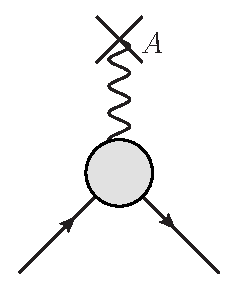
\includegraphics[scale=0.8]{eps/QED-static-field-blob} 
\end{minipage}
$	=	\hspace{2em} 	 $
\begin{minipage}{1.6in}
   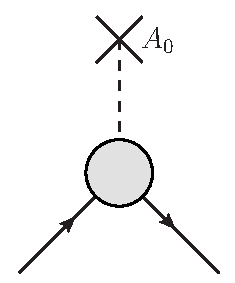
\includegraphics[scale=0.8]{eps/NRQED-static-coulomb-field}
\end{minipage}
$\hspace{2em}   +  \hspace{2em} $
\begin{minipage}{1.6in}
   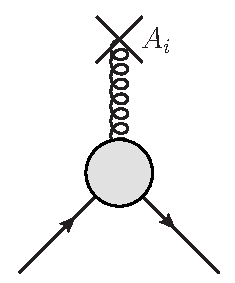
\includegraphics[scale=0.8]{eps/NRQED-static-vector-field} 
\end{minipage}
} 
\vspace{1em}

A general one-photon vertex in QED may be expressed in terms of form factors $F_1(q^2)$ and $F_2(q^2)$.  These encode all the information about radiative corrections, so the QED calculation here can conveniently be expressed with such factors.

The amplitude of scattering off a static vector potential is

%TODO check consisitency of \sigma^ij
\beq
e \bar{u}(p') \left[
	- \gv{\gamma} \cdot \v{A}(\v{q}) F_1 + \frac{i}{2m} \sigma^{ij} A^i q^j F_2 \right] u(p)
\eeq

or in terms of Pauli spinors instead, up to $1/m^3$

\beq
\begin{split}
=& 	F_1 \phis^\dagger \left[
	- \frac{e}{2m} (\v{p'} + \v{p} ) \cdot \v{A} - \frac{ie}{2m} \gv{\sigma} \cdot \v{q} \times \v{A}
	+ \frac{ie}{8m^3} (\v{p'}^2 + \v{p}^2 ) \gv{\sigma} \cdot \v{q} \times \v{A} \right ] \phis
 \\& 	+F_2 \phis^\dagger \left [ - \frac{ie}{2m} \gv{\sigma} \cdot \v{q} \times \v{A} 
	+ \frac{ie}{16m^3}  (\v{p'}^2 + \v{p}^2 ) \gv{\sigma} \cdot \v{q} \times \v{A}
	+ \frac{ie}{8m^3}  (\gv{\sigma}\cdot \v{p'})( \gv{\sigma} \cdot \v{q} \times \v{A})( \gv{\sigma} \cdot \v{p})  \right ] \phis
\end{split}
\eeq

For scattering off a static potential $A_0$

\beq
	e \bar{u}(p') \left [ 
		\gamma^0 A^0 F_1 - \frac{i}{2m} \sigma^{0j} A^0 q^j F_2 \right ] u(\v{p})
\eeq
Again expressing in terms of Pauli spinors
\beq \begin{split}
	=& F_1 \phis^\dagger \left [e A^0 - \frac{e}{8m^2} \v{q}^2 + \frac{ie}{4m^2} \gv{\sigma} \cdot (\v{p'} \times \v{p}) A^0 \right ] \phis
\\	& + F_2 \phis^\dagger \left [ - \frac{e}{8m^2}\v{q}^2  + \frac{ie}{4m^2} \gv{\sigma} \cdot (\v{p'} \times \v{p}) A^0 \right ] \phis		
\end{split}
\eeq

So the electron-external field scattering, as calculated in QED, has been expressed in terms of mostly nonrelativistic quantities.  There are still the form factors to expand, which depend on $q^2 = (q-0)^2 - \v{q}^2$.  But $q_0$ is of lower order than $\v{q}$, so the leading order corrections will involve only $\v{q}^2$.  They are

\beqa
	F_1(q^2) &=& 1 - \frac{ \alpha}{3\pi} \left [ \frac{ \v{q}^2}{m^2} \left( \ln\frac{m}{\lambda} \right ) \right ]	\\ 
	F_2(q^3) &=& a_e - \frac{\alpha}{\pi} \frac{\v{q}^2}{12m^2}	\\
\eeqa 
They contain an explicit dependence on the finite photon mass $\lambda$.

The first part of the calculation of scattering from the NRQED Lagrangian is straightforward --- only tree level vertices enter the calculation, so it can be read directly off the Lagrangian.  However, this would fix the coefficients as having a direct dependence on the photon mass, rather than, as one might expect, the value of the cut-off.  For instance, the coefficient of the Darwin term would be found to be
\beq
	c^{QED}_D = 1 + \frac{\alpha}{\pi}\frac{8}{3} \left[ \ln\big(\frac{m}{\lambda}\big)  - \frac{3}{8} \right]
\eeq

But of course, in calculating from NRQED at this level of precision perturbation theory terms will also enter. This introduces a further renormalization of the coefficients, in a similar manner to the production of counterterms in QED.  Without further correction these perturbations would spoil the agreement of QED and NRQED.  The solution is to introduce an additional term in the NRQED Lagrangian that simply subtracts off the unwanted term.

To again use the Darwin term as an example, it was found that in the absence of perturbation theory the value for $c_D$ labelled $c^{QED}_D$ would cause QED and NRQED to predict the same result.  However, when perturbations are taken into account there will be an {\it additional} contribution, of the same form of the Darwin term, with some coefficient we can call $c^{NRQED}_D$.  So the actual value of $c_D$ should be adjusted in order to bring the two theories back into agreement:
\beq
	c_D = c^{QED}_D - c^{NRQED}_D
\eeq

The particular value found for $c^{NRQED}_D$ is 
\beq
	c^{NRQED}_D = -\frac{\alpha}{\pi}\frac{8}{3} \left[ \ln\big(\frac{\lambda}{2 \Lambda}\big) + \frac{5}{6} \right ]
\eeq
Which means

\beq
	c_D = 1 + \frac{\alpha}{\pi} \frac{8}{3}\left[ \ln\big(\frac{m}{\lambda}\big)  - \frac{3}{8} + \frac{5}{6}\right]
\eeq

With the result that the final correction to this coefficient depends upon the cut-off, just as with the regular renormalization theory.  The same idea goes through to each other coefficient.


\subsection{Vertices}


To formally establish rules for the various vertices written above, it is necessary to strip off the external fields, and write derivatives of such fields in terms of their momentum.  The coulomb potential $A_0$ becomes a Coulomb photon, so (for example) $\grad \cdot \v{E}$ becomes the Darwin vertex, consisting of two fermion legs and a Coulomb photon, and a vertex with a factor of $-(e / 8m^2 ) \v{q}^2$.

Coulomb photon propagator

\VertexEq{nrqed-coulomb-photon-prop}
	{\frac{1}{\v{q}^2 + \lambda^2} }

Transverse photon propagator

\VertexEq{nrqed-transverse-photon-prop}
	{\frac{ \delta^{ij} - \frac{q^i q^j}{\v{q}^2 - \lambda^2} }{ (q^0)^2 - \v{q}^2 - \lambda^2 + ie} }


Darwin vertex

\VertexEq{Darwin-vertex}
	{\frac{-e}{8m^2} \abs{\v{p'} - \v{p}}^2}

Fermi vertex

\VertexEq{Fermi-vertex}
	{ \frac{ie}{2m} (\v{p'} - \v{p} ) \times \gv{\sigma} }
	
	